\chapter{Anexos}

\section{Ejemplos de consultas} 
\label{sec:ejemplos}

En este anexo del trabajo sen va a mostrar algunas preguntas que se le pueden realizar al
sistema desarrollado a modo de ilustrar su
funcionamiento.

\section{Consultas REST}

Voy a ilustrar distintas consultas utilizando el protocolo REST implementado. Algunas han sido realizadas desde la documentación OpenAPI y otras desde el programa \href{https://www.postman.com/}{Postman}\footnote{Es un aplicación que nos permite realizar consultas a APIs.}.

\vskip 0.4in

Consulta para obtener el total de defunciones
por Tuberculosis en España durante el año 2002 para los varones. \ref{fig:1}
\FloatBarrier
\begin{figure}[h]
	\centering
	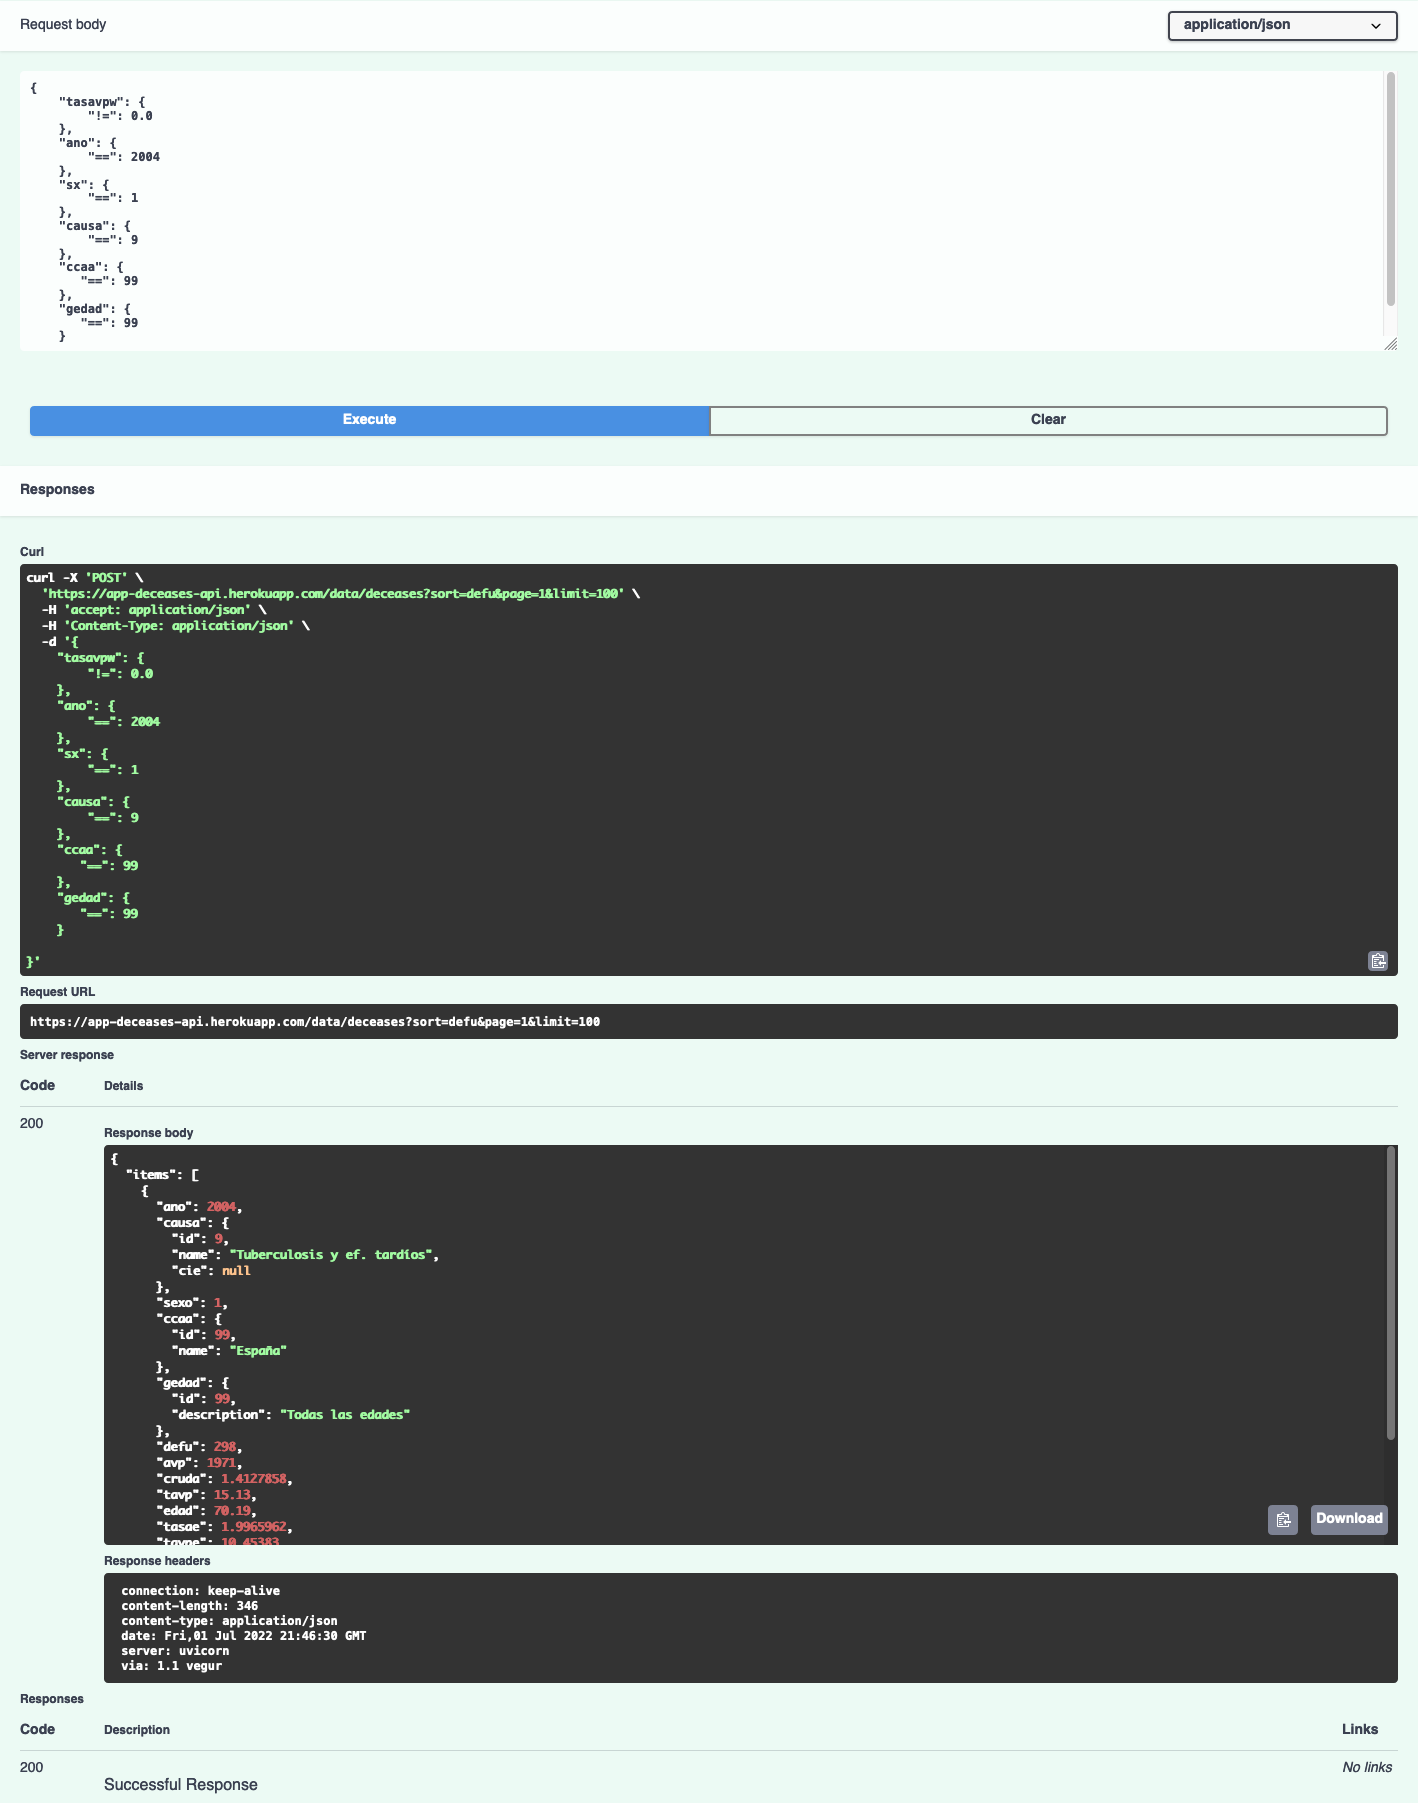
\includegraphics[width=\textwidth]{doc/logos/imgs/ejemplo1.png}
	\caption{ Consulta realizada a través de la documentación. }
	\label{fig:1}
\end{figure}
\FloatBarrier

Consulta realizada al manager de pronóstico sobre la evolución a 2 años de la causa de
muerte ``Paro cardíaco, muerte sin asistencia.''
Este manager a parte de ofrecer la gráfica también devuelve el conjunto de variables
estimadas. \ref{fig:2}
\FloatBarrier
\begin{figure}[h]
	\centering
	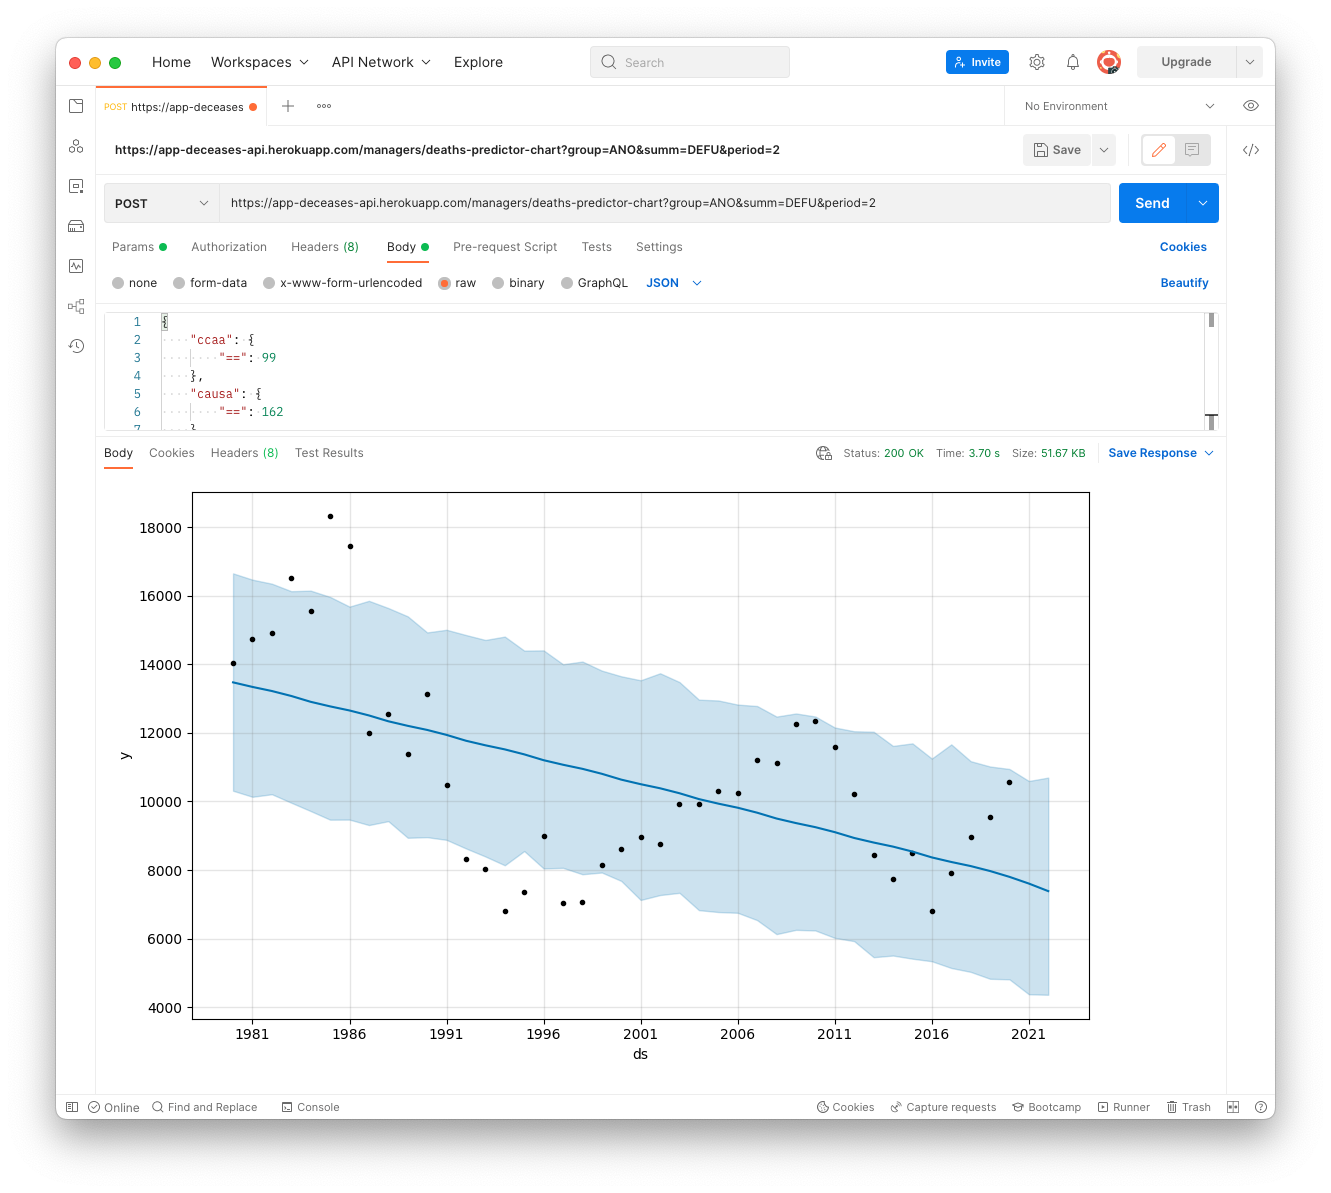
\includegraphics[width=\textwidth]{doc/logos/imgs/ejemplo2.png}
	\caption{ Consulta realizada a través de \href{https://www.postman.com/}{Postman}. }
	\label{fig:2}
\end{figure}
\FloatBarrier

Consulta realizada al manager de gráficos donde solicitamos una gráfica con la evolución 
de fallecimientos en toda España a causa del VIH. \ref{fig:3}
\FloatBarrier
\begin{figure}[h]
	\centering	
	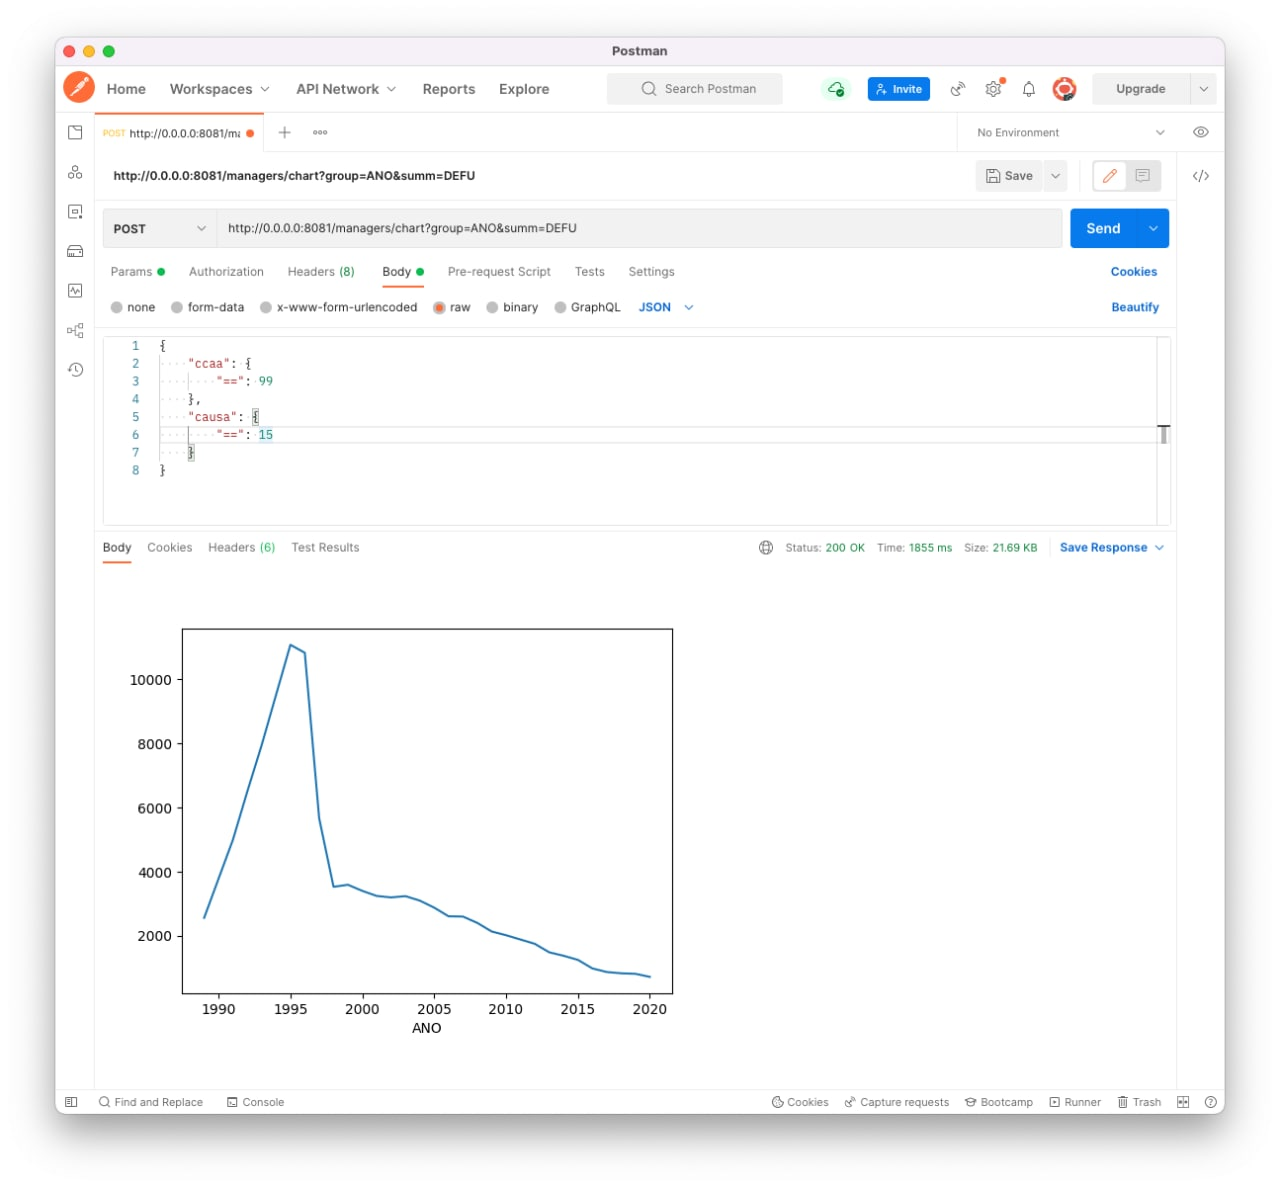
\includegraphics[width=\textwidth]{doc/logos/imgs/api-managers.jpg}
	\caption{ Llamada a POST /managers/chart desde
	\href{https://www.postman.com/}{Postman}. }
    \label{fig:3}
\end{figure}
\FloatBarrier

\section{GraphiQL}
Voy a ilustrar distintas consultas utilizando el lenguaje de consultas GraphQL. Se ha 
utilizado el IDE GraphiQL que incluye el proyecto. A continuación se puede apreciar el 
potencial de este tipo de consultas donde podemos proyectar únicamente los campos que 
son de nuestro interés y podemos obtener información de distintos recursos en una única llamada.

\vskip 0.4in

Query para obtener los datos de los repositorios: enfermedades disponibles, clasificación CIE y grupos de edad. \ref{fig:4}
\FloatBarrier
\begin{figure}[h]
	\centering
	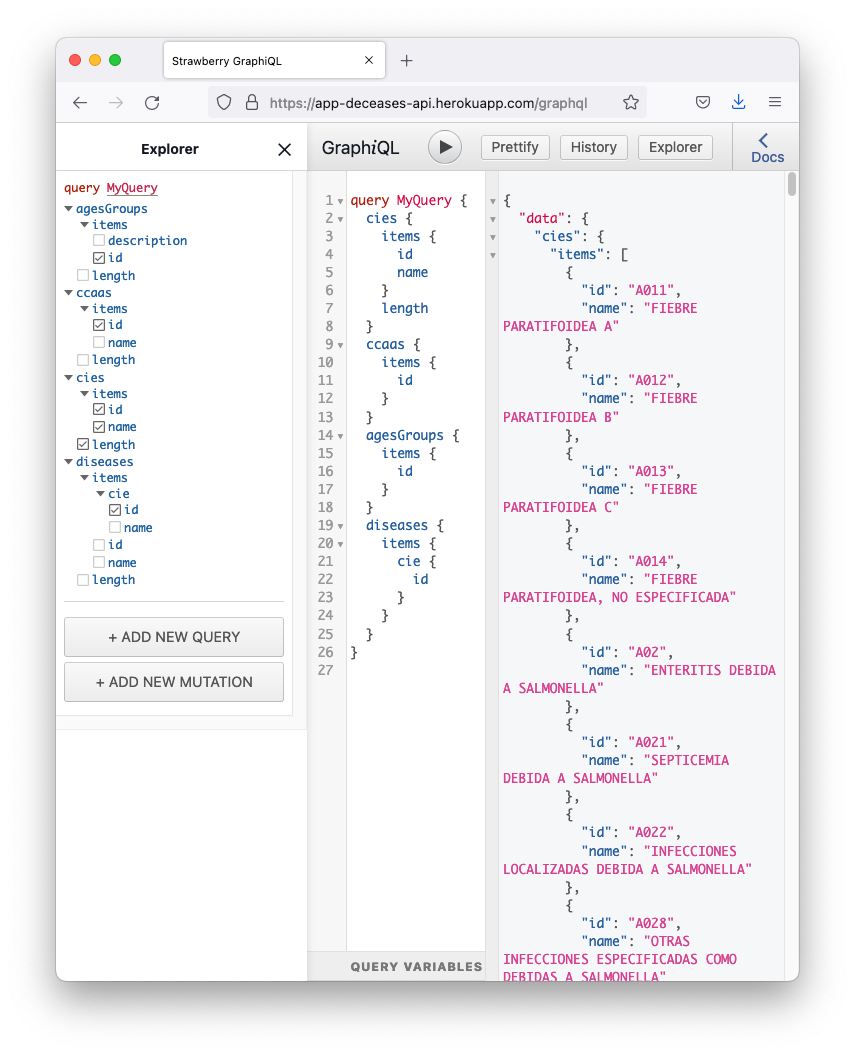
\includegraphics[width=0.85\textwidth]{doc/logos/imgs/ejemplo3.png}
	\caption{ Consulta realizada a través de GraphiQL. }
	\label{fig:4}
\end{figure}
\FloatBarrier

Ejemplo de una operación de tipo mutación para obtener los distintos tipos de cánceres que
clasifica con los que trabaja el sistema. Con parámetros personalizados proyectados y paginados. \ref{fig:5}
\FloatBarrier
\begin{figure}[h]
	\centering
	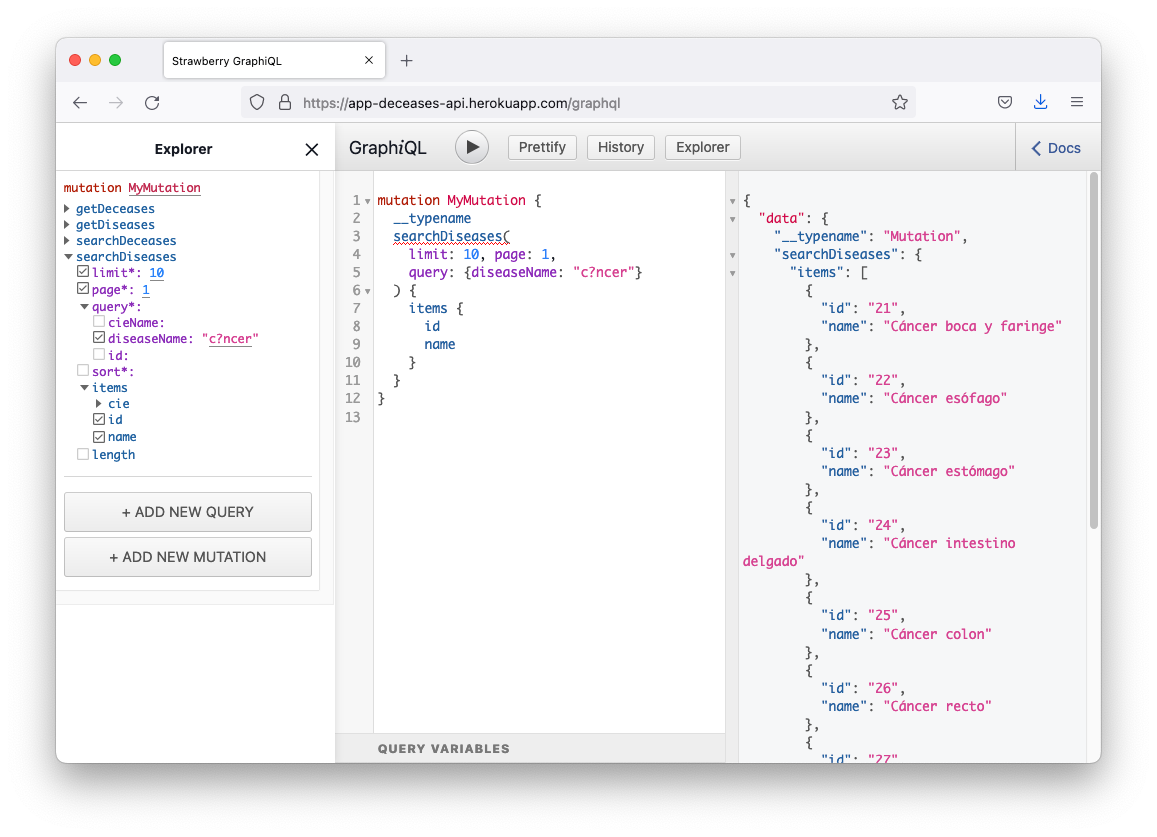
\includegraphics[width=\textwidth]{doc/logos/imgs/ejemplo4.png}
	\caption{ Mutación que obtiene los cánceres clasificados usando GraphiQL. }
	\label{fig:5}
\end{figure}
\FloatBarrier


En la siguiente mutación se están realizando dos operaciones. En primer lugar, buscando
todas las enfermedades registradas que tienen la palabra `ca|áncer'. En segundo lugar se
están solicitando las 10 causas con más fallecimientos que tiene más de 10 casos, a nivel
nacional, en todos los grupos de edad ocurridas durante 2008.
\begin{lstlisting}[caption=Ejemplo de mutación usando el protocolo GraphQL] 
mutation MyMutation {
    __typename
    searchDiseases(query: {diseaseName: "c?ncer"}) {
        items {
            name
        }
    }
    getDeceases(query: {
        defu: {gt: 100}, 
        ccaa: {eq: 99}, 
        ano: {eq: 2008}, 
        gedad: {eq: 99}
    }, limit: 10, sort: "defu") {
        length
        items {
            defu
            causa {
                name
            }
            ccaa {
                name
            }
        }
    }
}
\end{lstlisting}


En esta consulta estamos realizando dos mutaciones (la descrita arriba) y además solicitamos: la comunidad autónoma,
el número de defunciones y la edad media de la CCAA con más defunciones por Cáncer de boca
y faringe durante el año 2018. \ref{fig:6}
\FloatBarrier
\begin{figure}[h]
	\centering
	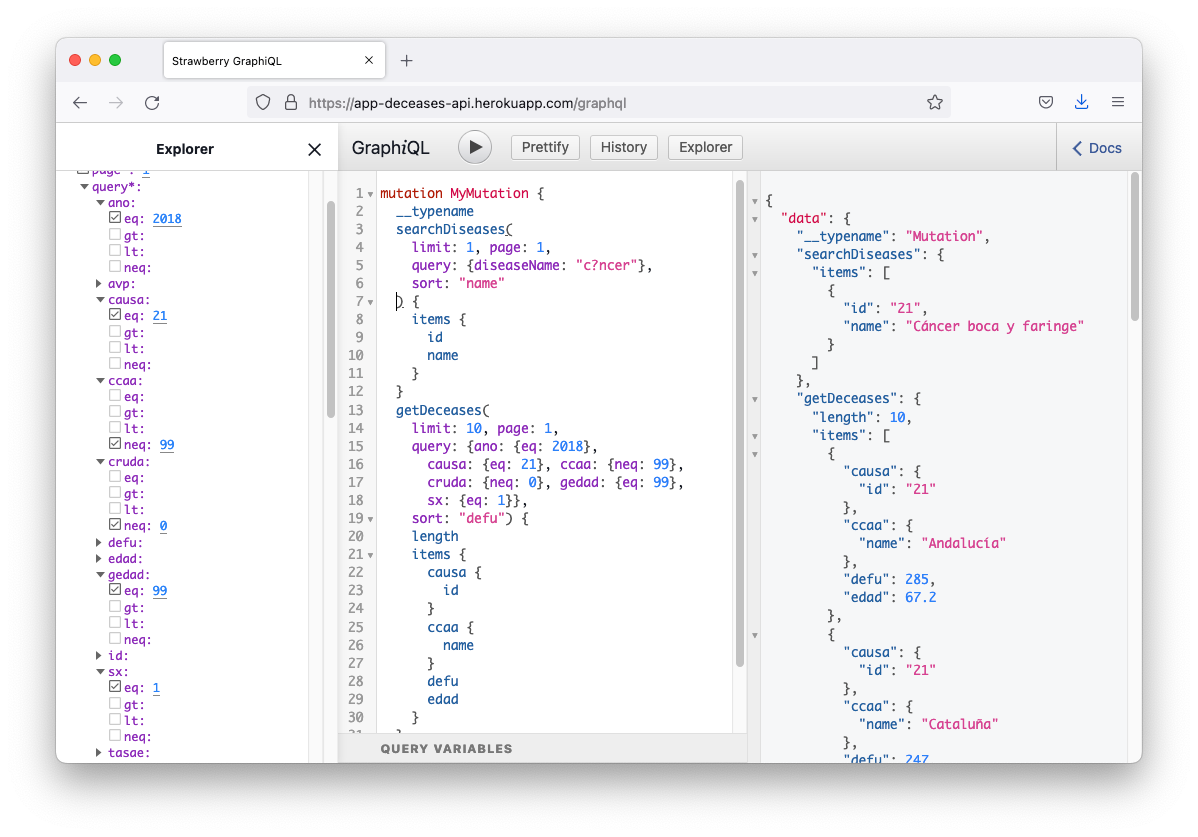
\includegraphics[width=\textwidth]{doc/logos/imgs/ejemplo5.png}
	\caption{ Mutación agrupadas GraphQL. }
		\label{fig:6}
\end{figure}
\FloatBarrier
